% This is TBP on Ag(100):
\label{sec:single-TBP-Ag100}
%%%%%%%%%%%%%%%%%%%%%%%%%%%%%%%%%%%%%%%%%%%%%%%%%%%%%%%%%
Molecules are adsorbed on Ag(100) at RT. The resulting conglomerates are shown in \autoref{fig:single-TBP-Ag100-RT}. The very most surface area is covered with unregular patterns. The step edges are covered, assuming a sufficient large mobility at RT to move from the terrace to the nearest step edge. The only free step edges observed are due to tip formings on the sample surface since these are created after the molecules are stuck on the surface because of the low temperatures during measurement.
%%%%%%%%%%%%%%%%%%%%%%%%%% Annealing %%%%%%%%%%%%%%%%%%%%%%%%%%%%%%%%%%%%%
\paragraph{Annealing}
The RT adsorption is annealed to \SI{170}{\celsius} for \SI{10}{\min} and investigated in LT-STM again (\autoref{fig:single-TBP-Ag100-annealed}). No big changes are visible, neither in the formation of new assemblies nor in the distribution of molecules at terraces or at step edges. No chain formation could be observed.

\begin{figure}[] \centering
	\subfigure[Adsorption at RT]{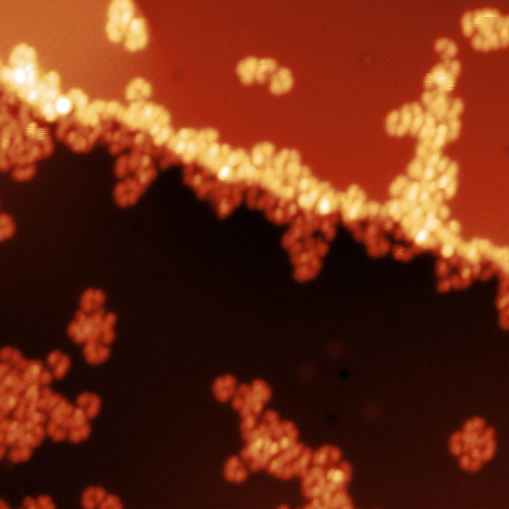
\includegraphics[width=0.45\textwidth]{./images/F150615-121334-cut.png}
		\label{fig:single-TBP-Ag100-RT}
	}
	\subfigure[RT adsorption annealed to \SI{170}{\celsius} for \SI{10}{\min}]{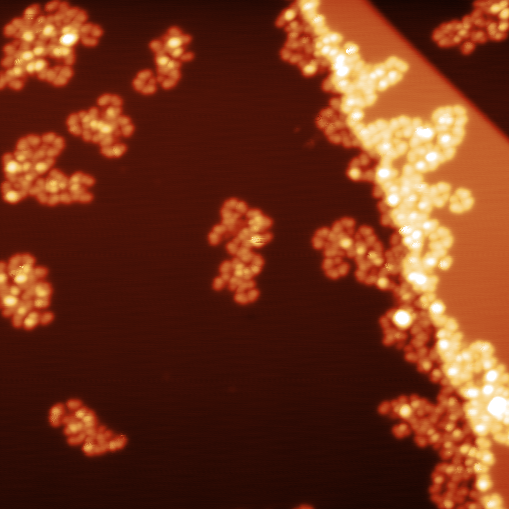
\includegraphics[width=0.45\textwidth]{./images/F150616-102758-44nm.png}
		\label{fig:single-TBP-Ag100-annealed}
	}
	\caption{Annealing after RT adsorption of molecules on Ag(100). \subref{fig:single-TBP-Ag100-RT} STM data of molecules adsorbed at RT (Scan parameters: $U_b=\SI{1}{\volt}, I_t=\SI{0,03}{\nano \ampere}$), \subref{fig:single-TBP-Ag100-annealed} After annealing for \SI{10}{\min} to \SI{170}{\celsius} (Scan parameters: $U_b=\SI{1}{\volt}, I_t=\SI{0,1}{\nano \ampere}$). Color scale \SIrange{0}{600}{\pico\meter}. Image width: \SI{44}{\nm}.}
	\label{fig:single-TBP-Ag100-annealing}
\end{figure}

%%%%%%%%%%%%%%%%%%%%%%%%%% Assembly models %%%%%%%%%%%%%%%%%%%%%%%%%%%%%%%%%%%%%
\paragraph{Assembly}
Since no regular self-assembled islands are present on the surface, more detail is put on the only repeating binding motifs on this surface. One of this configurations resembles a cross (\autoref{fig:single-TBP-Ag100-cross}), while the second one is a variation of the dimer motif (\autoref{fig:single-TBP-Ag100-doubledimer}).

%%%%%%%%%%%%%%%%%%%%%%%% Dimer %%%%%%%%%%%%%%%%%%%%%%%%%%%%%%%%

While on copper, two molecules may form a dimer in head-to-head of head-to-tail configuration, on silver some form tetramers from two parallel merged dimers. While one dimer looks like two ``U'''s with facing open ends ($\in \ni$), the other dimer is shifted to closely match the first dimer best and lies parallel.

%\begin{figure}[] \centering
%
%	\caption{Dimer configuration of TBP adsorbed on Ag(100) at RT. \subref{fig:single-TBP-Ag100-dimer} STM data. Scan parameters: $U_b=\SI{0.328}{\volt}, I_t=\SI{0.035}{\nano \ampere}$, color scale \SIrange{0}{300}{\pico\meter}. Image width: \SI{5}{\nm}. \subref{fig:single-TBP-Ag100-dimer-model} Model representation in the same size.}
%	\label{fig:single-TBP-Ag100-dimer}
%\end{figure}

%%%%%%%%%%%%%%%%%%%%%%%% Double Dimer %%%%%%%%%%%%%%%%%%%%%%%%%%%%%%%%
\begin{figure}[] \centering
	\subfigure[]{  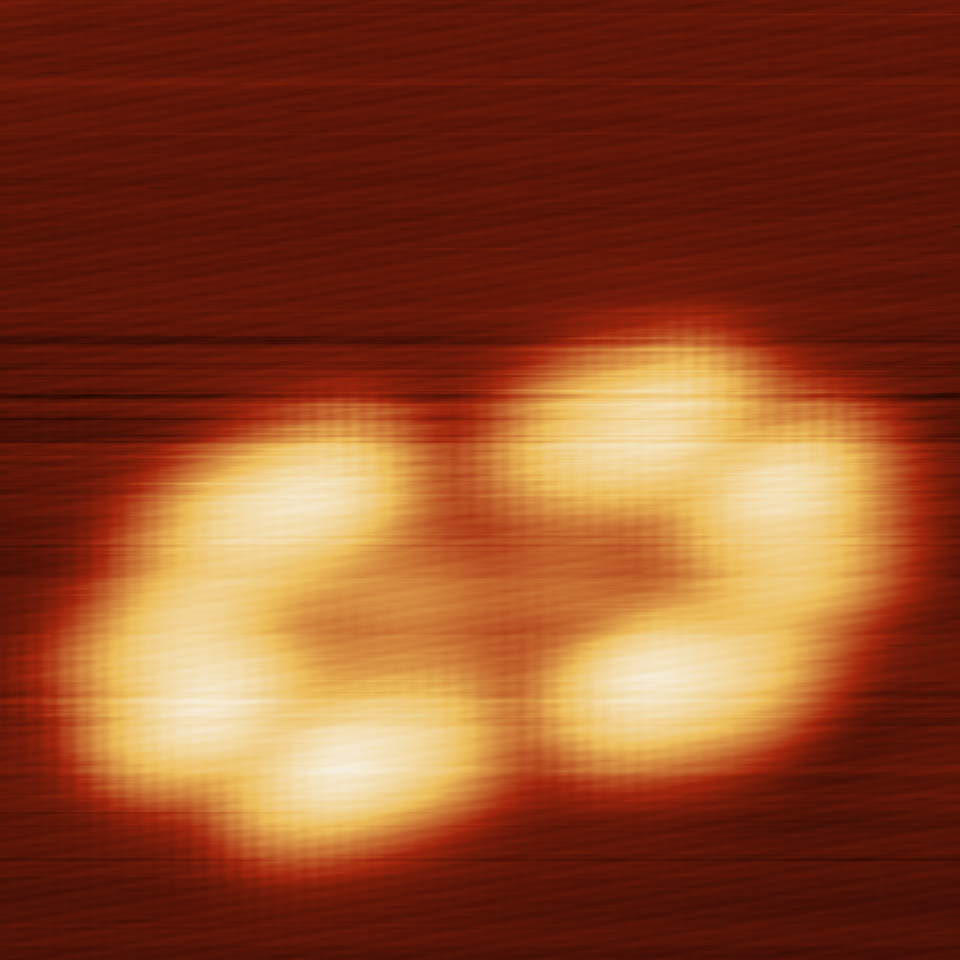
\includegraphics[width=0.3\textwidth]{./images/F150612-153409-5nm.png}
	\label{fig:single-TBP-Ag100-dimer-STM}
	}
	\subfigure[]{  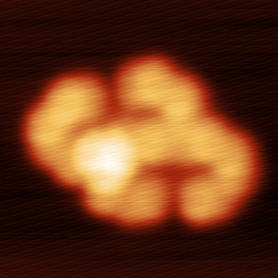
\includegraphics[width=0.3\textwidth]{./images/F150612-144915-6nm.png}
		\label{fig:single-TBP-Ag100-doubledimer-STM}
	}
	\subfigure[]{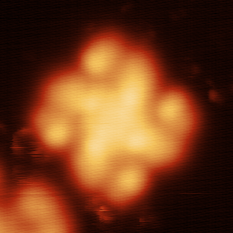
\includegraphics[width=0.3\textwidth]{./images/F150612-154558-10nm.png}
	\label{fig:single-TBP-Ag100-cross-STM}
	}
	\subfigure[]{  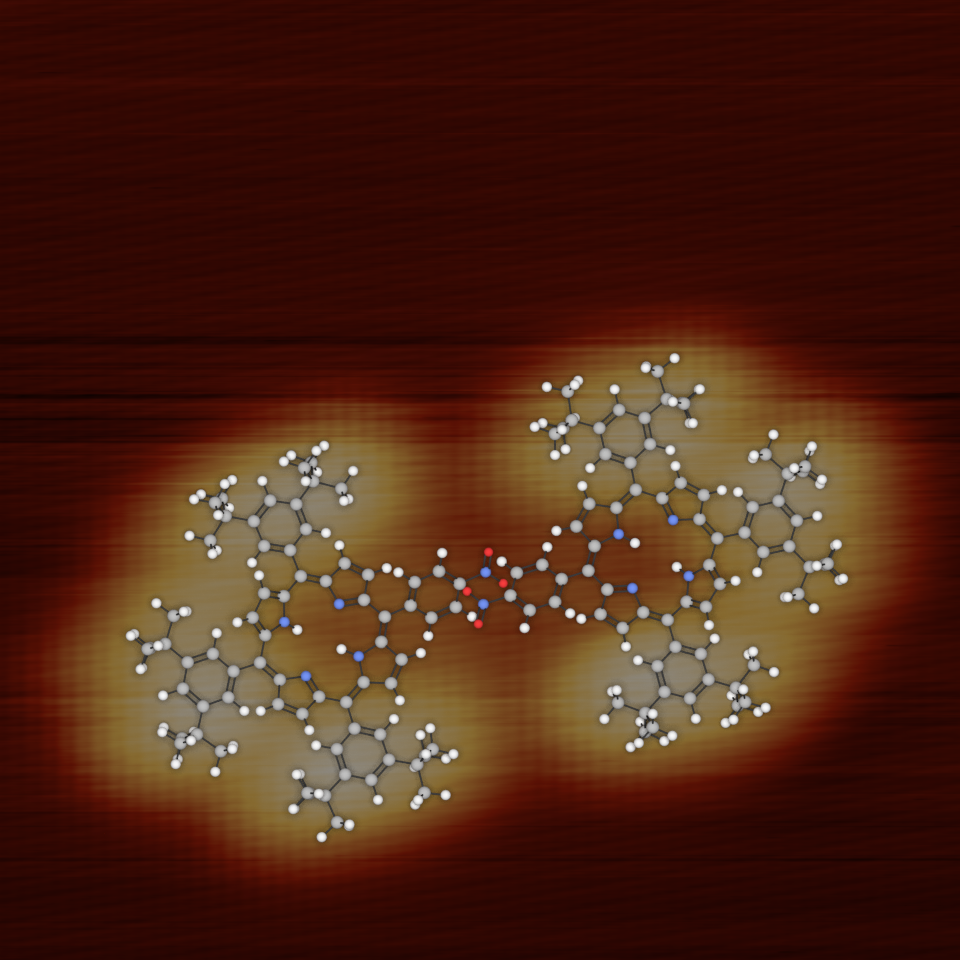
\includegraphics[width=0.3\textwidth]{./images/F150612-153409-5nm-model.png}
	\label{fig:single-TBP-Ag100-dimer-model}
	}
	\subfigure[]{  \includegraphics[width=0.3\textwidth]{./images/F150612-144915-6nm-model}
		\label{fig:single-TBP-Ag100-doubledimer-model}
	}
	\subfigure[]{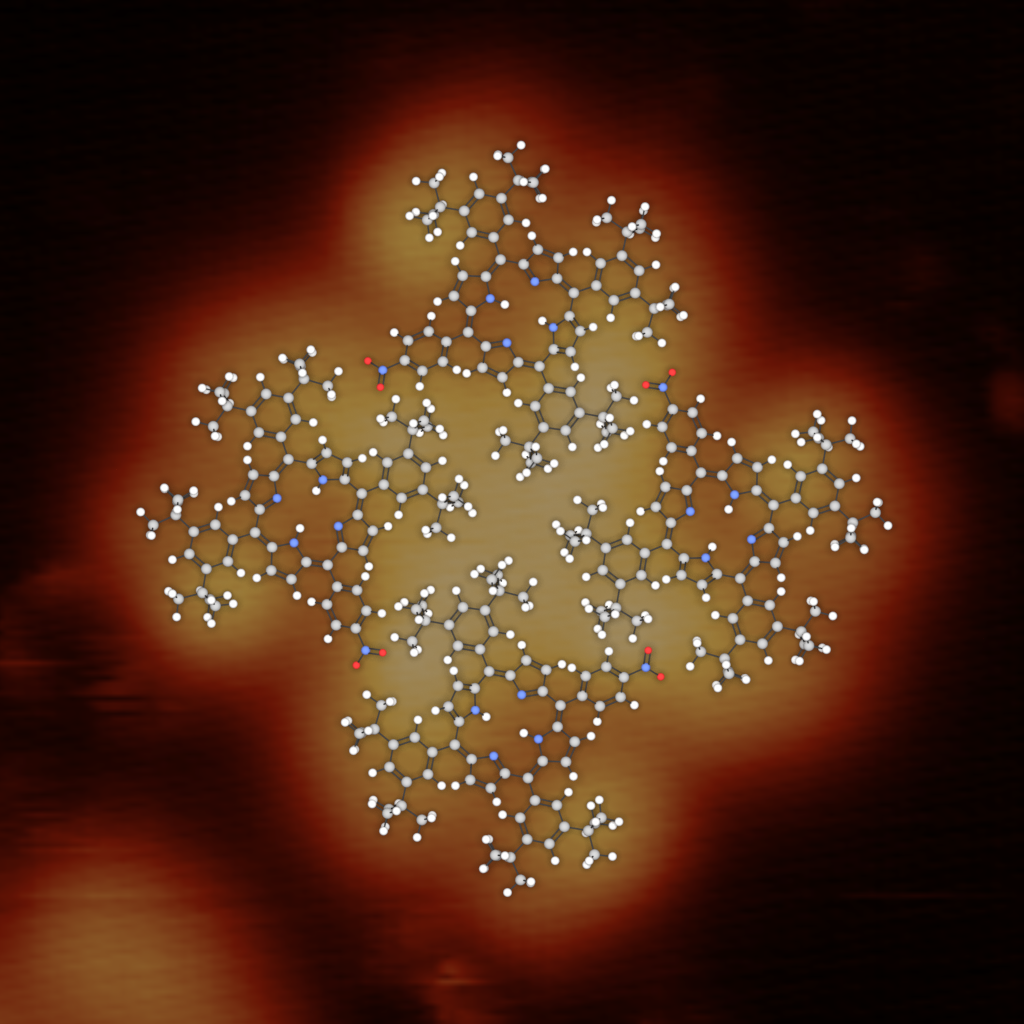
\includegraphics[width=0.3\textwidth]{./images/F150612-154558-10nm-model3.png}
	\label{fig:single-TBP-Ag100-cross-model}
	}
	\caption{Different observed binding configurations of TBP adsorbed on Ag(100) at RT. \subref{fig:single-TBP-Ag100-dimer-STM} STM data of dimer configuration. Scan parameters: $U_b=\SI{0.328}{\volt}, I_t=\SI{0.035}{\nano \ampere}$, Image width: \SI{5}{\nm}. \subref{fig:single-TBP-Ag100-dimer-model} Model representation. \subref{fig:single-TBP-Ag100-doubledimer-STM} STM data of two coalescent dimers. Scan parameters: $U_b=\SI{0.097}{\volt}, I_t=\SI{0.035}{\nano \ampere}$, Image width: \SI{6}{\nm}. \subref{fig:single-TBP-Ag100-doubledimer-model} Model representation. \subref{fig:single-TBP-Ag100-cross-STM} A cross consisting of four TBP molecules. Scan parameters: $U_b=\SI{2.3}{\volt}, I_t=\SI{0,035}{\nano \ampere}$, Image width: \SI{10}{\nm}. \subref{fig:single-TBP-Ag100-cross-model} Model representation. Color scale in all STM images \SIrange{0}{300}{\pico\meter}}
	\label{fig:single-TBP-Ag100-doubledimer}
\end{figure}
%%%%%%%%%%%%%%%%%%%%%%%% Cross %%%%%%%%%%%%%%%%%%%%%%%%%%%%%%%%
Another motif looks like a cross and shown in \autoref{fig:single-TBP-Ag100-cross}. Build out of four molecules, wherer each is rotated by \SI{90}{\degree} with respect to its preliminary neighbor. One can distinguish four di-tert-butyl groups from the central cross. Although there is no atom directly in the center, the cross looks bright in its center (in STM), which is somehow counterintuitive. 

%\begin{figure}[] \centering
%
%	\caption{\subref{fig:single-TBP-Ag100-cross-STM} A cross consisting of four TBP molecules. Scan parameters: $U_b=\SI{2.3}{\volt}, I_t=\SI{0,035}{\nano \ampere}$, color scale \SIrange{0}{300}{\pico\meter}. Image width: \SI{10}{\nm}. \subref{fig:single-TBP-Ag100-cross-model} Model representation in the same size.}
%	\label{fig:single-TBP-Ag100-cross}
%\end{figure}

\paragraph{Flexible Tert-Butyl-Functions}
\autoref{fig:single-TBP-Ag100-doubledimer-STM} shows an interesting feature of the tert-butyl functions.

\begin{itemize}
 \item Butyl groups within TBP feature different contrasts (look rotated), while the orientation of the butyl-groups doesn't follow the close packed substrate rows. ---------------- find image and explain
 \item TBP molecules have been heated on silver substrate for \SI{10}{\minute} at \SI{170}{\celsius}. The resulting sample did not feature chain-formation or improved ordering.
\end{itemize}

%%%%%%%%%%%%%%%%%% Single ordered area => Appendix? %%%%%%%%%%%%%%%%%%%%
%-------------- Add graphic to explain!-------------- 

%%%%%%%%%%%%%%%%%% Spectra %%%%%%%%%%%%%%%%%%%%
\paragraph{Spectroscopy}
\textcolor{red}{\textbf{
Some spectroscopy could be achieved that shows different typical features for different areas in the molecule. Note that the spectra were done for molecules sitting on a Ag(100) surface.
There is a clear indication, that the macrocycle of the molecule contributes to the broad peak in the dI/dV data at around \SI{1}{\V}, while the nitro groups dominate the spectra at around \SI{600}{\milli \V}. 
Look at the corresponding .pptx file for the spectra and the corresponding IGOR-files dimer/quatermer1-2 for the spectra.
}}